\section{Representation Statistics and Additional Visualizations}
\label{app:e}

\subsection{Statistical units and weighted PCA}
\label{subsec:e1}

For frame \(i\), modality \(m\), and location \(p\), let \(x_{im}^p\) denote a representation and \(\mathcal P_i\) the GT foreground locations. Equation~\eqref{eq:e1} defines the frame-mean vector \(\mu_{im}\) and the mean matched-location cosine \(s_i^{mn}\). Weather-group cosines average \(s_i^{mn}\) equally over frames. This differs both from taking the cosine of frame-mean vectors and from pooling all patches with equal patch weights. All 10,065 analyzed frames contain valid foreground, totaling 642,649 foreground spatial locations. Table~\ref{tab:e1} separates modality pairs.

\begin{equation}
\mu_{im}=\frac{1}{|\mathcal P_i|}\sum_{p\in\mathcal P_i}x_{im}^p,\qquad
s_i^{mn}=\frac{1}{|\mathcal P_i|}\sum_{p\in\mathcal P_i}\operatorname{cos}(x_{im}^p,x_{in}^p).
\label{eq:e1}
\end{equation}

Input, Shared, and Specific each have a separately fitted PCA basis. Within each representation type, all modalities and weather groups share that basis. PCA is fitted to \(\mu_{im}\), weighting each vector by \(1/(|\mathcal W|N_wM)\), where \(N_w\) is its weather-group frame count and \(M=3\). The leading two eigenvectors of the weighted centered covariance are used, without per-vector normalization or channel standardization. Each weather group and modality therefore contributes equally to fitting. Different representation columns have different bases and scales, so absolute Euclidean distances are not compared across columns.

The seven-weather scatter plot displays up to 400 frames per weather group, including all 383 overcast frames. Displayed frame indices are shared across modalities and representation panels; centroids and density contours use all frames. With the random seed and PCA bases fixed, we do not refit for visual separation, add jitter, or clip outliers. Figure~\ref{fig:e1} expands the main PCA visualization to all weather groups.

\subsection{High-dimensional similarity distributions and weather variation}
\label{subsec:e2}

Table~\ref{tab:e1} shows that Specific features are not approximately orthogonal for every modality pair: C--R cosines remain around 0.65 across the seven weather groups, while pairs involving LiDAR vary more across groups. This is compatible with the relative organization encouraged by the two branches and does not require modality-specific features to contain no information in common.

Figure~\ref{fig:e2} and Table~\ref{tab:e2} further show frame-level similarity distributions. The L--R Shared medians are 0.9632 in normal weather and 0.9662 in heavy snow. For Specific, the 5th--95th percentile range changes from 0.2113--0.4948 to 0.2578--0.7363. Violin width represents empirical density; thick and thin intervals show the 25th--75th and 5th--95th percentiles. These describe across-frame variability, not confidence intervals.

As an aggregation-sensitivity check, equal weighting of sequences gives mean cross-modal Specific cosines of approximately 0.440/0.584 in normal/heavy-snow conditions, compared with 0.446/0.537 under equal frame weighting. Shared features retain high consistency, while the precise Specific difference depends on aggregation weights. Weather is associated with sequence, scene, and object composition. High cosine values also cannot exclude a common dominant direction or low variance. These statistics are therefore interpreted together with component ablations, rather than as independent proof of semantic identifiability or a causal weather effect.

\textbf{Frame-level correspondence controls.} Figure~\ref{fig:e-correspondence} compares cosines of foreground-mean vectors for the same frame and for different-sequence frames within the same weather group, using ten fixed permutation seeds. Matched scores use the same retained anchors. Before centering, Shared C--L, C--R, and L--R cosines are 0.979214/0.970201/0.987697 for matched pairs and 0.979205/0.970225/0.987136 for mismatches. After subtracting each modality's weather-group mean, the matched/mismatched L--R values are 0.148740/\(-0.014689\), while the camera-related matched values remain close to zero. Thus, a common mean direction can account for much of the high uncentered frame-level similarity. This check does not resolve patch-level correspondence because frame averaging discards local information; it also does not isolate the contribution of the Shared branch. It is a control on the interpretation of similarity, rather than proof of either semantic decomposition or branch redundancy.

\subsection{Construction of gate and detection visualizations}
\label{subsec:e3}

Main-text Figure~\ref{fig:4} presents three scenes with camera predictions, complete LiDAR BEV and gate maps, and gate detail windows. Foreground/background gate means are 0.213/0.128, 0.259/0.115, and 0.288/0.118 from top to bottom. Full maps cover forward \(x\in[0,72]\) m and lateral \(y\in[-6.4,6.4]\) m; detail windows span 14\(\times\)8.4 m. The gate uses the native 16\(\times\)90 array and a common [0,1] scale without smoothing. Camera panels show the selected target's GT, while BEV and gate panels retain all GT references within the displayed region. GT overlays and regional statistics are added after feature-based prediction; no prior detector provides the gate.

Figure~\ref{fig:e-gate-examples} separately retains the seven-weather gate examples selected from 21 complete-gate candidates for scene readability, object arrangement, and local responses. During that export, GT fields were withheld at the fusion-module input and used only afterward. One historical candidate with unexplained repeated-inference differences was excluded. Table~\ref{tab:e3} summarizes these seven appendix examples, not the three main-text scenes. Figure~\ref{fig:e-gate-statistics} adds the full-test analysis: equally weighted frame-level foreground/background gate means are 0.2701/0.1176, and foreground means exceed background means in 99.06\% of frames. Selected examples and full-test statistics have different sampling units and are reported separately.

Figure~\ref{fig:e-comparison} compares strictly loaded released ASF and final ObjDec checkpoints on identical test frames, using FP32, batch size 1, the same detection postprocessing, and a score\(>0.3\) filter. Input-tensor hashes and GT were checked for all 20 candidates in the paired visualization pool. Original camera images, sequence-specific calibration, intrinsics, and distortion are retained. Both methods use identical camera crops, complete BEV ranges, and 12\(\times\)6 m BEV detail windows. The selected objects' maximum geometric 3D IoUs among retained predictions change from 0.572/0.000/0.000 to 0.719/0.476/0.741 from top to bottom. These values are neither AP nor the official one-to-one matching outcome; the middle example remains below IoU 0.5.

Figure~\ref{fig:e3} adds heavy- and light-snow examples: the selected objects' maximum 3D IoUs change from 0.095 to 0.728 and from 0.354 to 0.223, respectively. The latter also has a locally high gate response, illustrating that foreground-related activation is insufficient to determine final box accuracy. The complete 20-frame candidate atlas is retained as an archival asset; it is not repeated in the manuscript. Selected qualitative cases do not estimate aggregate detection gains.

\begin{table}[tbp]
\centering
\caption[Full-set similarity by modality pair]{\textbf{Full-set similarity by modality pair.} Cosines in the original 256-dimensional space are averaged over matched foreground locations within each frame, then equally over frames within a weather group.}
\label{tab:e1}
\begingroup
\footnotesize
\setlength{\tabcolsep}{3pt}
\renewcommand{\arraystretch}{1.22}
\begin{tabularx}{\linewidth}{@{}>{\hsize=1.50943\hsize\linewidth=\hsize\raggedright\arraybackslash}X>{\hsize=0.94340\hsize\linewidth=\hsize\centering\arraybackslash}X>{\hsize=0.94340\hsize\linewidth=\hsize\centering\arraybackslash}X>{\hsize=0.94340\hsize\linewidth=\hsize\centering\arraybackslash}X>{\hsize=0.94340\hsize\linewidth=\hsize\centering\arraybackslash}X>{\hsize=0.94340\hsize\linewidth=\hsize\centering\arraybackslash}X>{\hsize=0.94340\hsize\linewidth=\hsize\centering\arraybackslash}X>{\hsize=0.94340\hsize\linewidth=\hsize\centering\arraybackslash}X>{\hsize=0.94340\hsize\linewidth=\hsize\centering\arraybackslash}X>{\hsize=0.94337\hsize\linewidth=\hsize\centering\arraybackslash}X@{}}
\toprule
\textbf{Weather} & \textbf{Frames} & \textbf{Seqs.} & \textbf{FG patches} & \textbf{Shared C--L} & \textbf{Shared C--R} & \textbf{Shared L--R} & \textbf{Specific C--L} & \textbf{Specific C--R} & \textbf{Specific L--R} \\
\midrule
Normal & 4309 & 17 & 317581 & 0.9455 & 0.9584 & 0.9621 & 0.3429 & 0.6545 & 0.3410 \\
Overcast & 383 & 2 & 33918 & 0.9520 & 0.9574 & 0.9676 & 0.4211 & 0.6501 & 0.4111 \\
Fog & 1049 & 6 & 43909 & 0.9391 & 0.9505 & 0.9647 & 0.4659 & 0.6612 & 0.4572 \\
Rain & 1317 & 8 & 125257 & 0.9431 & 0.9565 & 0.9586 & 0.3855 & 0.6511 & 0.3767 \\
Sleet & 1106 & 7 & 41665 & 0.9584 & 0.9478 & 0.9638 & 0.5112 & 0.6529 & 0.4840 \\
Light snow & 803 & 4 & 36196 & 0.9470 & 0.9582 & 0.9622 & 0.4787 & 0.6590 & 0.4643 \\
Heavy snow & 1098 & 7 & 44123 & 0.9525 & 0.9481 & 0.9601 & 0.4954 & 0.6458 & 0.4693 \\
\bottomrule
\end{tabularx}
\endgroup
\end{table}

\begin{table}[tbp]
\centering
\caption[L--R similarity quantiles]{\textbf{L--R similarity quantiles.} Each observation is a frame-level mean of matched-patch cosines. Quantiles describe variation across frames, not confidence intervals.}
\label{tab:e2}
\begingroup
\footnotesize
\setlength{\tabcolsep}{3pt}
\renewcommand{\arraystretch}{1.22}
\begin{tabularx}{\linewidth}{@{}>{\hsize=1.23077\hsize\linewidth=\hsize\raggedright\arraybackslash}X>{\hsize=1.23077\hsize\linewidth=\hsize\raggedright\arraybackslash}X>{\hsize=1.23077\hsize\linewidth=\hsize\raggedright\arraybackslash}X>{\hsize=0.76923\hsize\linewidth=\hsize\centering\arraybackslash}X>{\hsize=0.76923\hsize\linewidth=\hsize\centering\arraybackslash}X>{\hsize=0.76923\hsize\linewidth=\hsize\centering\arraybackslash}X@{}}
\toprule
\textbf{Weather} & \textbf{Branch} & \textbf{Pair} & \textbf{Median} & \textbf{5th percentile} & \textbf{95th percentile} \\
\midrule
normal & common & LiDAR--4D Radar & 0.9632 & 0.9433 & 0.9776 \\
normal & unique & LiDAR--4D Radar & 0.3384 & 0.2113 & 0.4948 \\
heavysnow & common & LiDAR--4D Radar & 0.9662 & 0.9141 & 0.9806 \\
heavysnow & unique & LiDAR--4D Radar & 0.4538 & 0.2578 & 0.7363 \\
\bottomrule
\end{tabularx}
\endgroup
\end{table}

\begin{table}[tbp]
\centering
\caption[Frame-level statistics of the seven appendix gate examples]{\textbf{Frame-level statistics of the seven appendix gate examples.} Each frame has 1,440 complete patches. Foreground regions use GT footprints expanded by 0.7 m after prediction. Values summarize seven qualitative examples, not weather-wide means.}
\label{tab:e3}
\begingroup
\footnotesize
\setlength{\tabcolsep}{3pt}
\renewcommand{\arraystretch}{1.22}
\begin{tabularx}{\linewidth}{@{}>{\hsize=1.36585\hsize\linewidth=\hsize\raggedright\arraybackslash}X>{\hsize=1.36585\hsize\linewidth=\hsize\raggedright\arraybackslash}X>{\hsize=0.85366\hsize\linewidth=\hsize\centering\arraybackslash}X>{\hsize=0.85366\hsize\linewidth=\hsize\centering\arraybackslash}X>{\hsize=0.85366\hsize\linewidth=\hsize\centering\arraybackslash}X>{\hsize=0.85366\hsize\linewidth=\hsize\centering\arraybackslash}X>{\hsize=0.85366\hsize\linewidth=\hsize\centering\arraybackslash}X@{}}
\toprule
\textbf{Weather} & \textbf{Frame ID} & \textbf{GT objects} & \textbf{FG patches} & \textbf{FG gate mean} & \textbf{BG gate mean} & \textbf{FG \(-\) BG} \\
\midrule
Normal & seq20\_rdr00628 & 1 & 28 & 0.3154 & 0.1208 & 0.1946 \\
Overcast & seq13\_rdr00146 & 2 & 60 & 0.2995 & 0.1112 & 0.1883 \\
Fog & seq39\_rdr00582 & 1 & 40 & 0.2942 & 0.1078 & 0.1864 \\
Rain & seq25\_rdr00154 & 4 & 142 & 0.2882 & 0.1181 & 0.1702 \\
Sleet & seq50\_rdr00456 & 2 & 65 & 0.2913 & 0.1179 & 0.1734 \\
Light snow & seq43\_rdr00169 & 1 & 35 & 0.3711 & 0.1103 & 0.2608 \\
Heavy snow & seq55\_rdr00385 & 1 & 35 & 0.2817 & 0.1186 & 0.1631 \\
\bottomrule
\end{tabularx}
\endgroup
\end{table}

\begin{figure}[p]
\centering
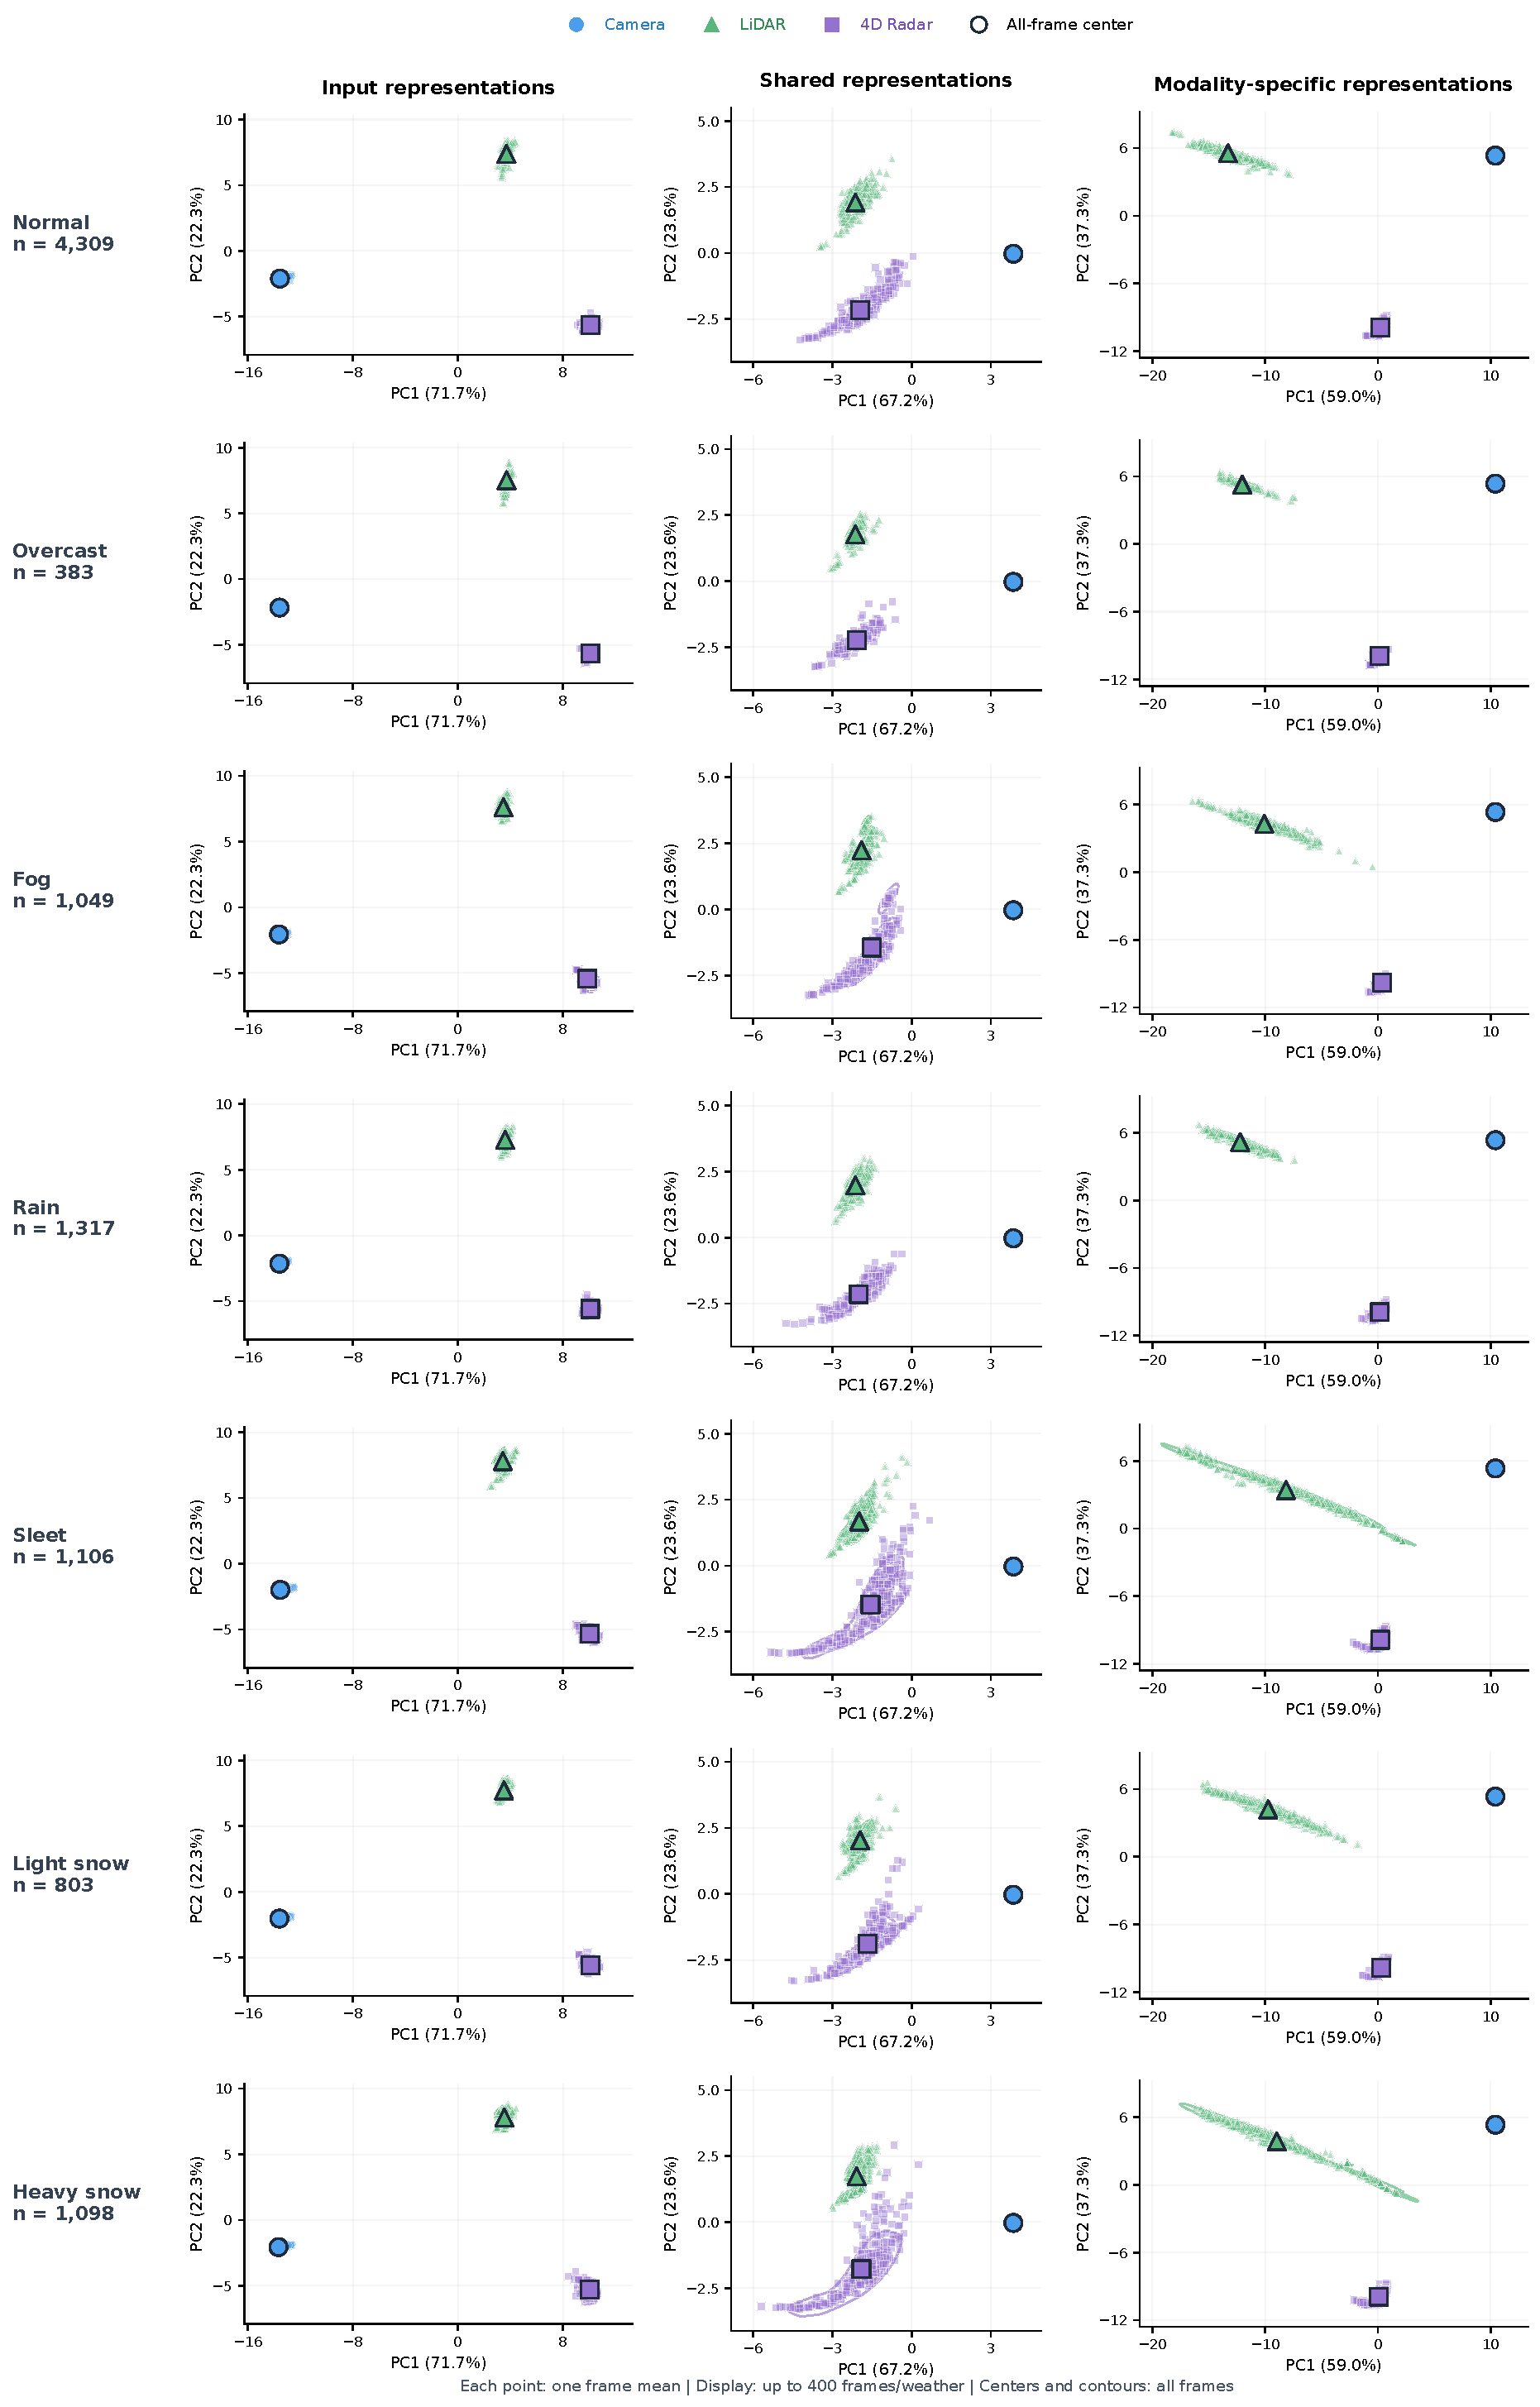
\includegraphics[width=\linewidth,height=.69\textheight,keepaspectratio]{assets/pca_all_weather.pdf}
\caption{Frame-level representation distributions over the complete K-Radar v1 test set. Rows indicate weather groups; columns show input, shared, and modality-specific representations. Each point is a frame's mean vector over GT foreground locations, projected using the fixed weighted PCA basis for its column. Blue circles, green triangles, and purple squares denote camera, LiDAR, and 4D radar. Up to 400 frames are displayed per group, including all 383 overcast frames. Large outlined markers and density contours use all frames, and n denotes the full group size. Each column shares its basis and axis ranges across weather; columns are fitted independently. Residual modality structure in these projections and high-dimensional cosine consistency in Table~\ref{tab:e1} characterize different properties.}
\label{fig:e1}
\end{figure}

\begin{figure}[p]
\centering
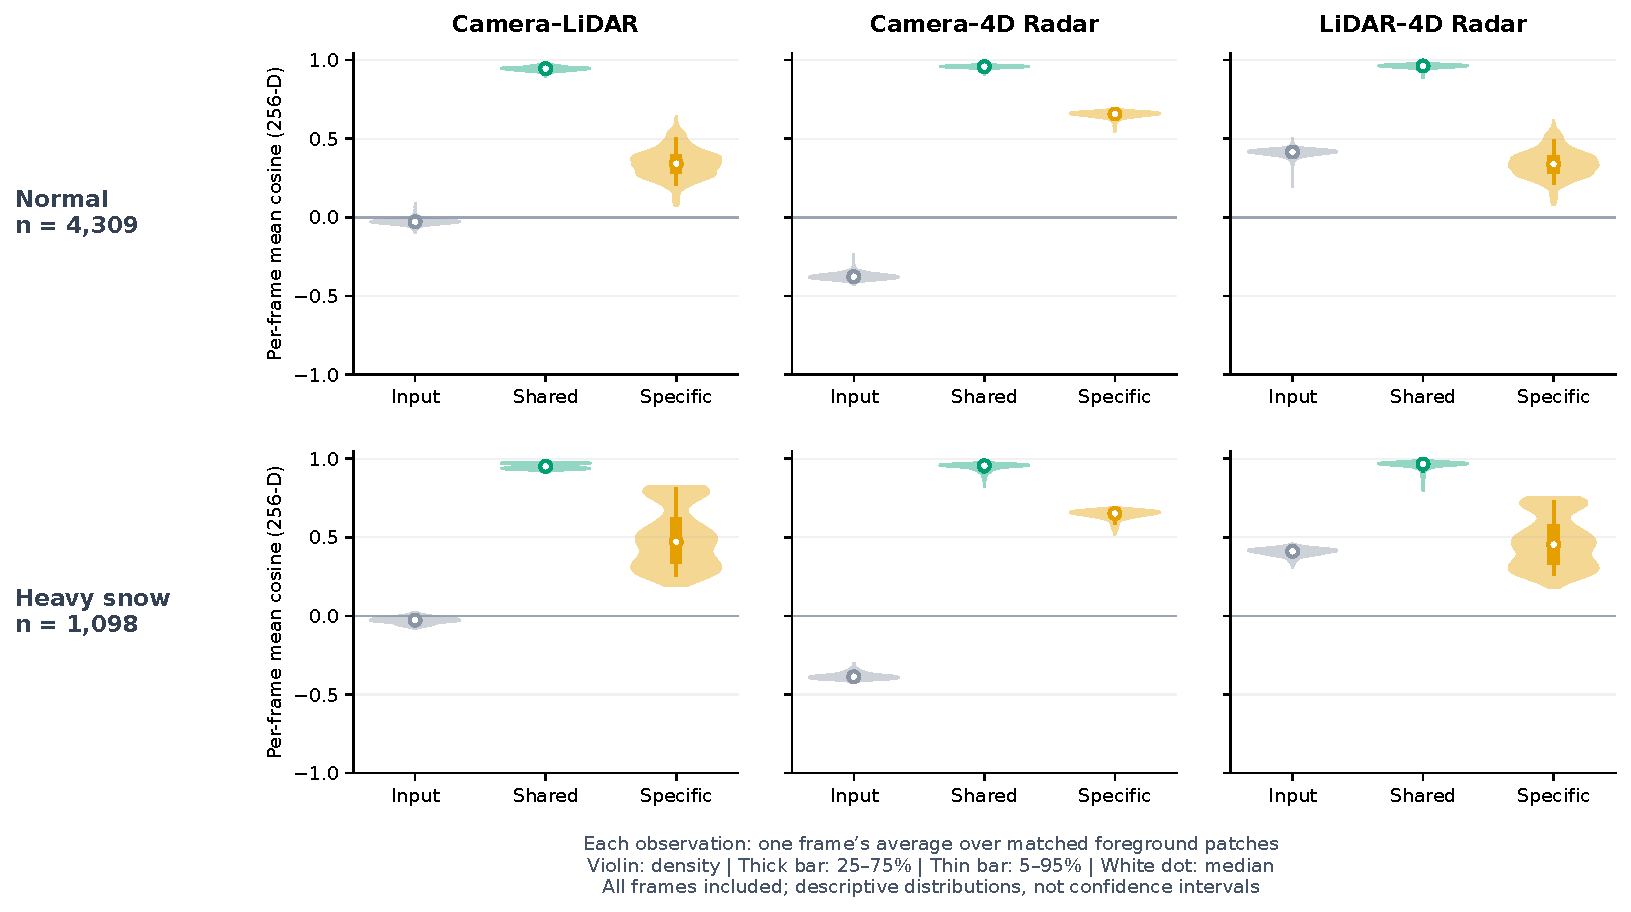
\includegraphics[width=\linewidth,height=.69\textheight,keepaspectratio]{assets/similarity_distributions.pdf}
\caption{Cosine-similarity distributions in the original 256-dimensional space for three sensor pairs under normal weather and heavy snow. Each observation is the mean matched-foreground-patch cosine within a frame, including all 4,309 and 1,098 frames. Gray, green, and yellow indicate input, shared, and modality-specific representations. Violins show empirical density, white points show medians, and thick/thin intervals span the 25th--75th/5th--95th percentiles, rather than confidence intervals for estimated means. Shared features concentrate at high similarity, while specific-feature distributions vary by modality pair and weather. Similarities are not computed from PCA coordinates.}
\label{fig:e2}
\end{figure}

\begin{figure}[p]
\centering
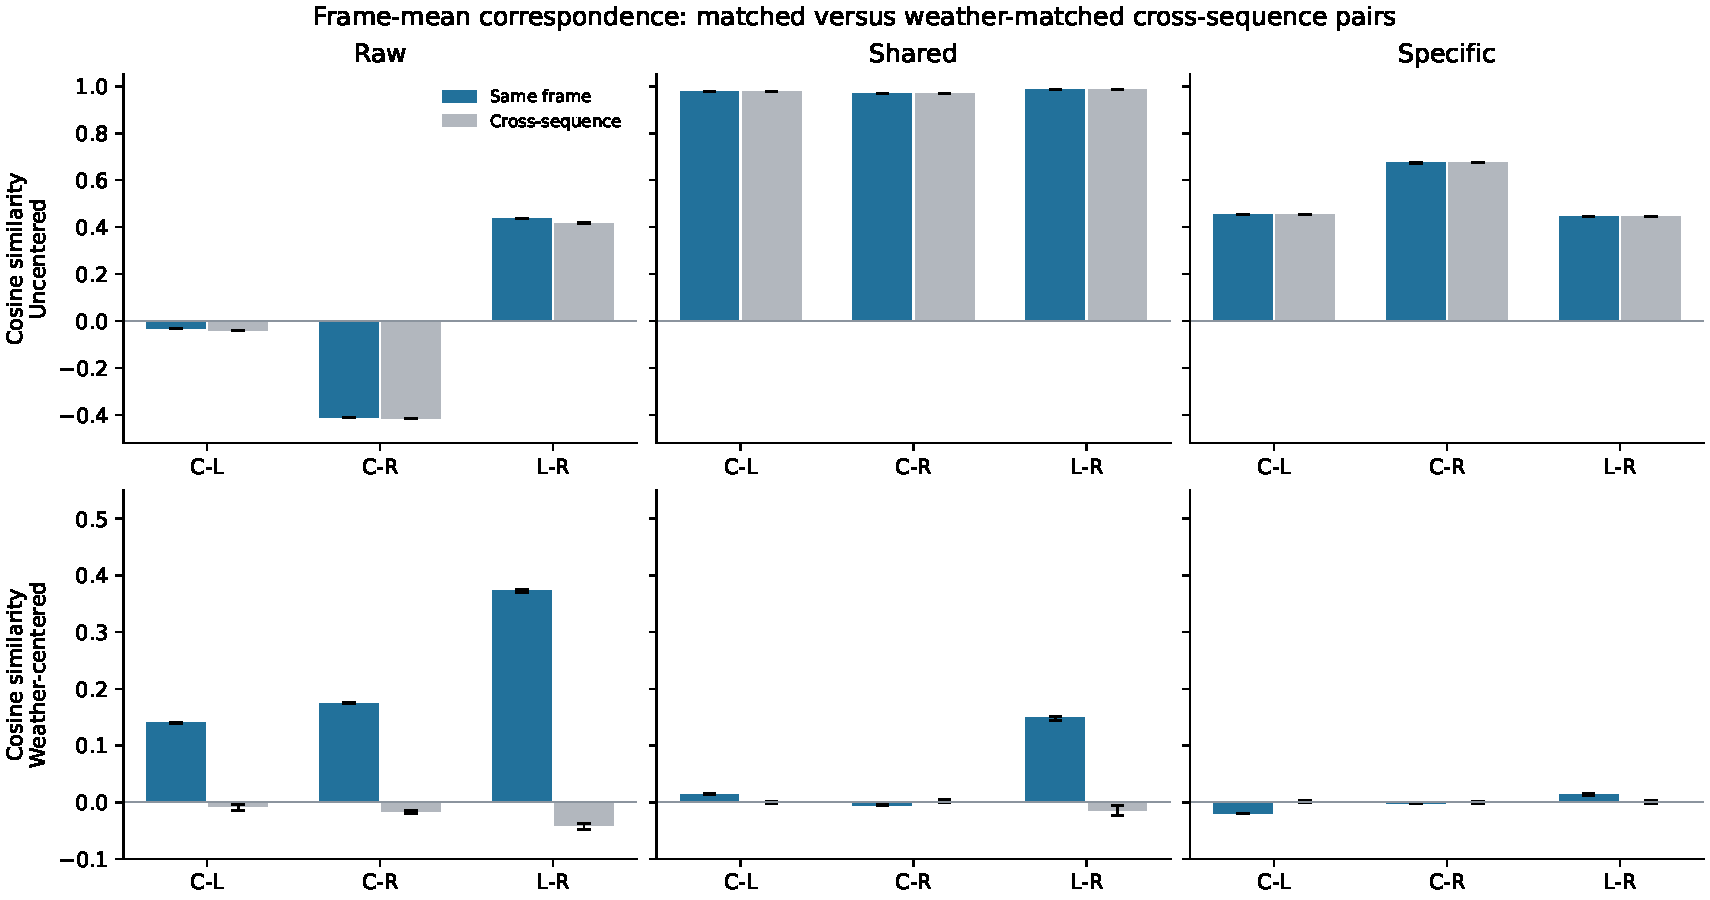
\includegraphics[width=\linewidth,height=.65\textheight,keepaspectratio]{assets/frame_correspondence.pdf}
\caption{Frame-level cross-modal correspondence controls using foreground-mean vectors in the original feature space. Same-frame pairs are compared with different-sequence pairs from the same weather group over ten fixed permutation seeds; matched scores use the same retained anchors. Weather-centered results subtract the mean for each modality, representation type, and weather group before computing cosine similarity. These are cosines of frame-mean vectors, unlike the averages of matched-patch cosines in Figure~\ref{fig:e2}. Seed variation concerns mismatch sampling, not independently trained models. High uncentered shared cosine persists under mismatching, so high similarity alone does not demonstrate semantic correspondence.}
\label{fig:e-correspondence}
\end{figure}

\begin{figure}[p]
\centering
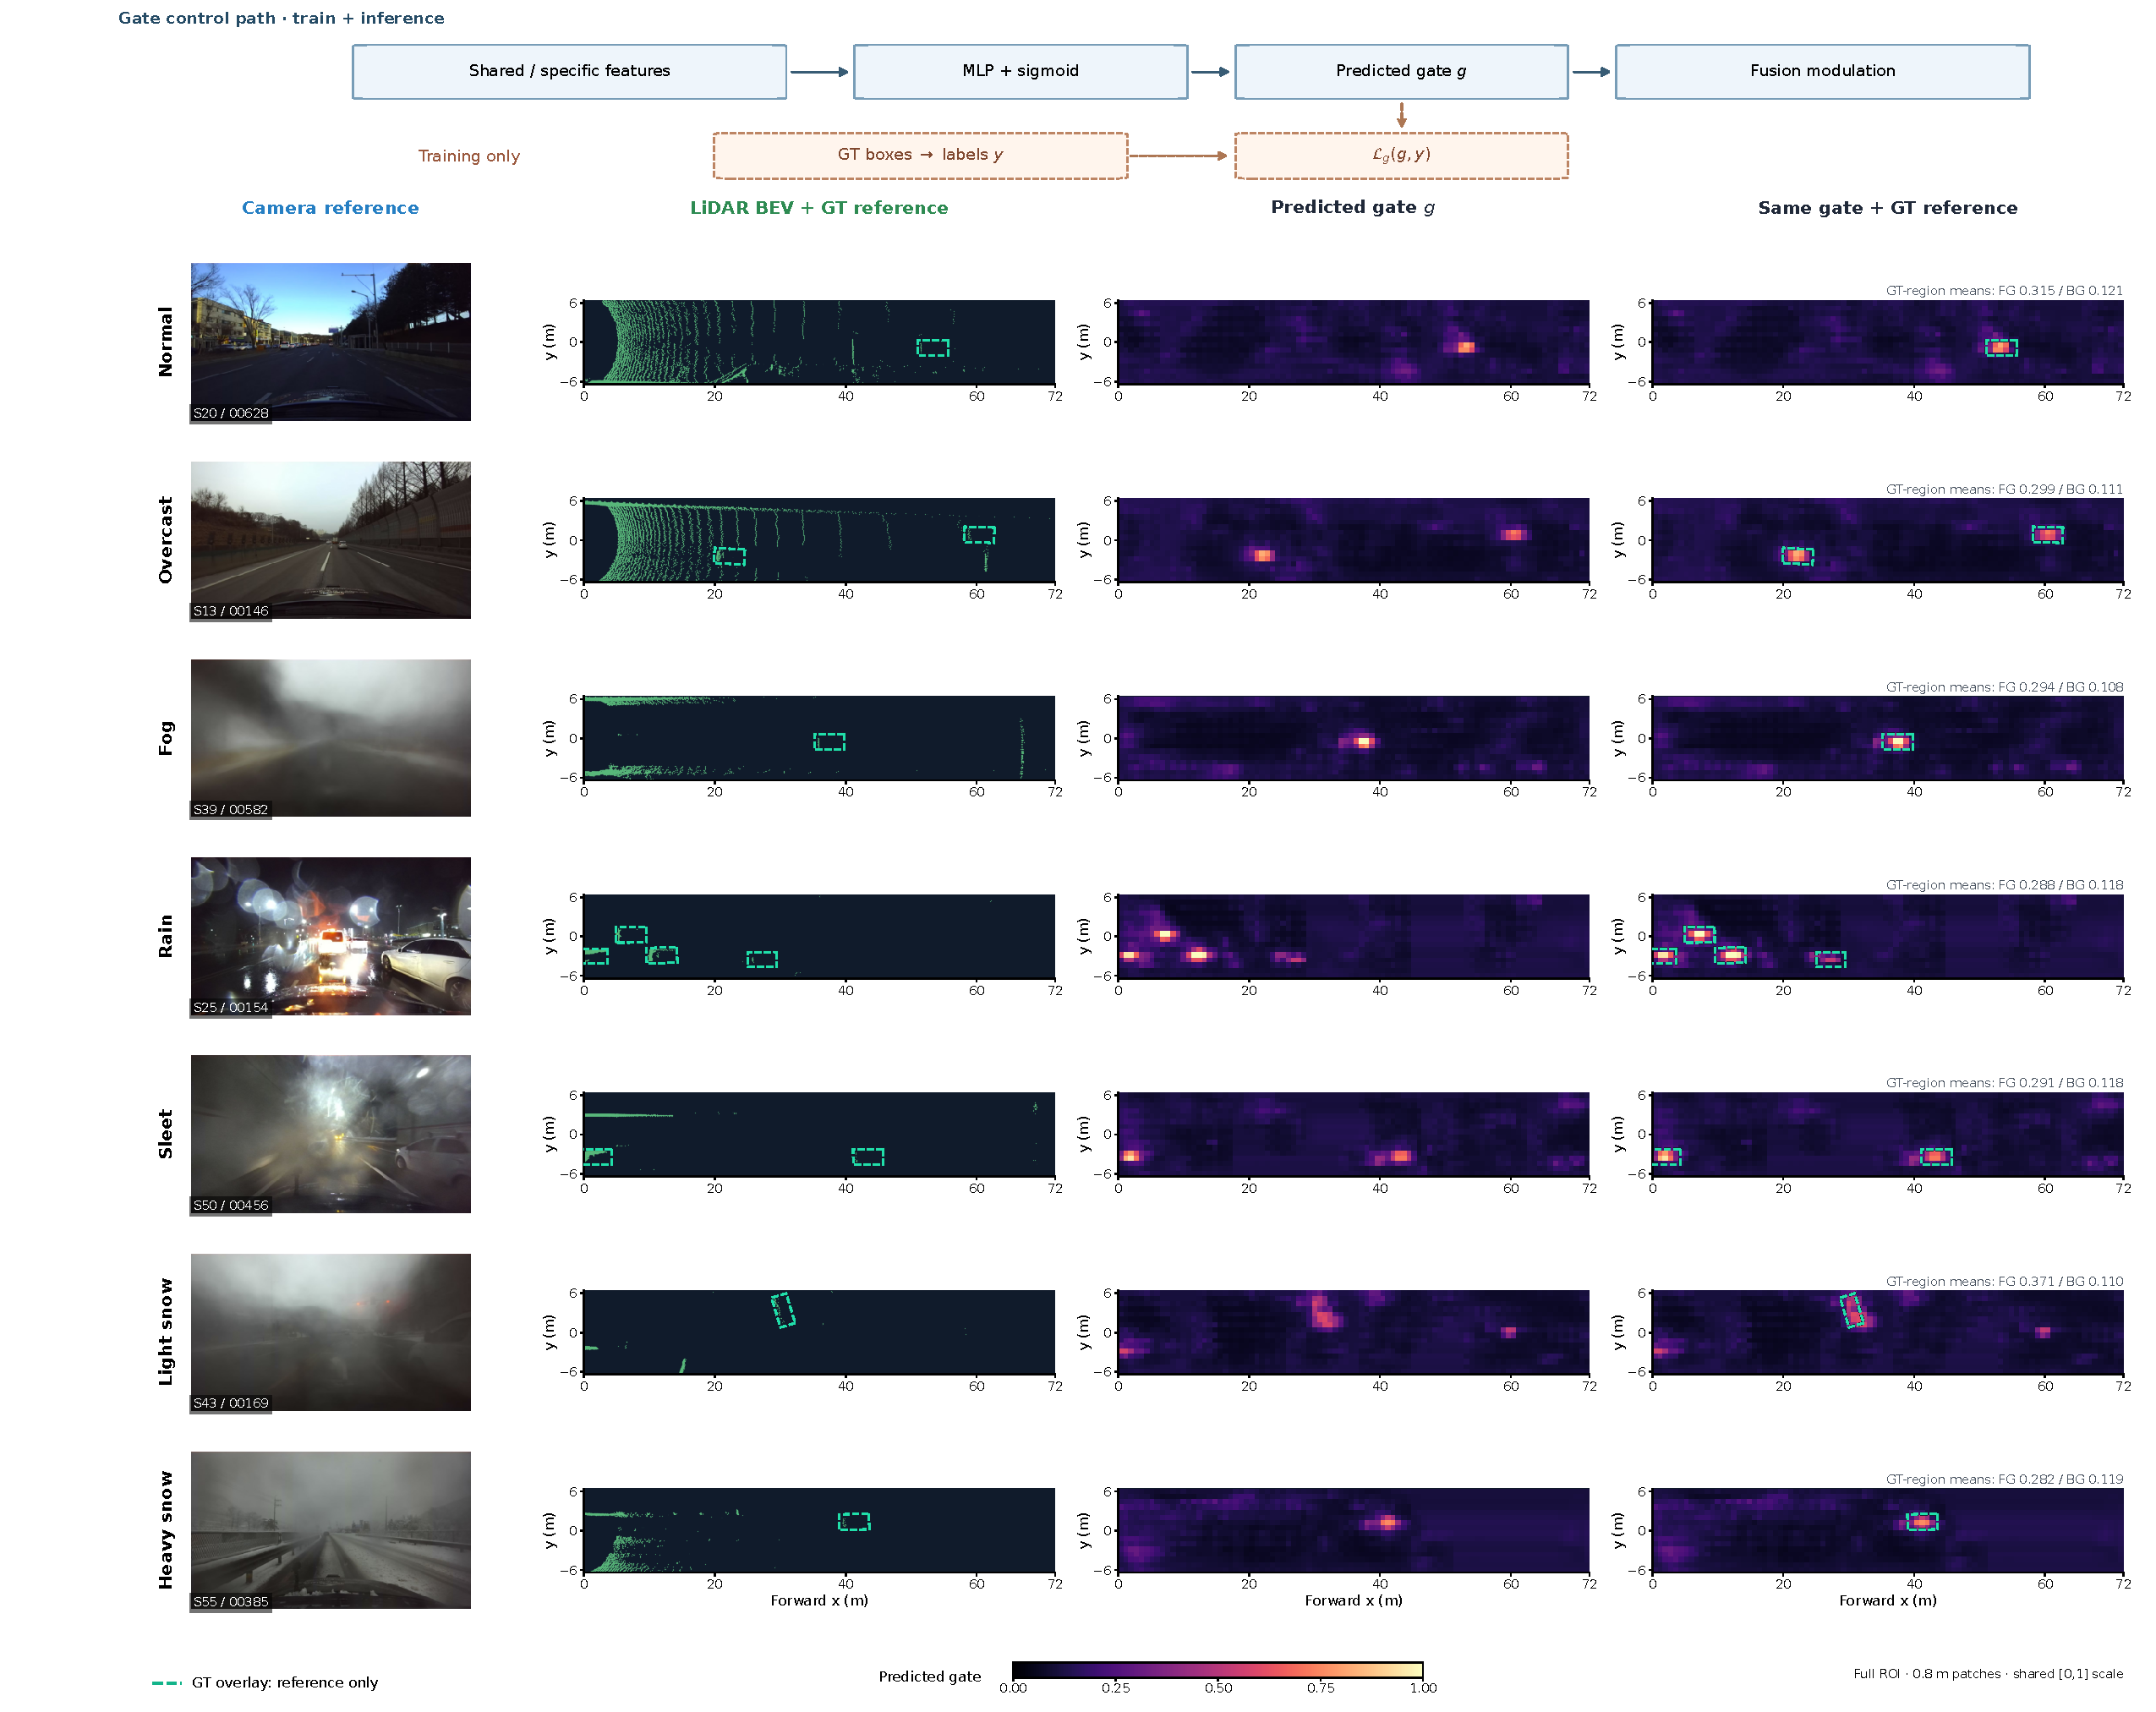
\includegraphics[width=\linewidth,height=.69\textheight,keepaspectratio]{assets/gate_all_weather_examples.pdf}
\caption{Additional spatial-gate examples across seven weather groups. Each example shows the camera reference, LiDAR BEV, the predicted gate, and the identical gate with GT references added after prediction. All gates use the native 16\(\times\)90 grid, 0.8 m patches, and a common [0,1] color scale without smoothing or per-frame normalization. Gates are predicted from input features; GT supplies only training labels and post-hoc visualization or statistics. These selected examples do not estimate weather-wide performance. Table~\ref{tab:e3} reports their frame-level statistics.}
\label{fig:e-gate-examples}
\end{figure}

\begin{figure}[p]
\centering
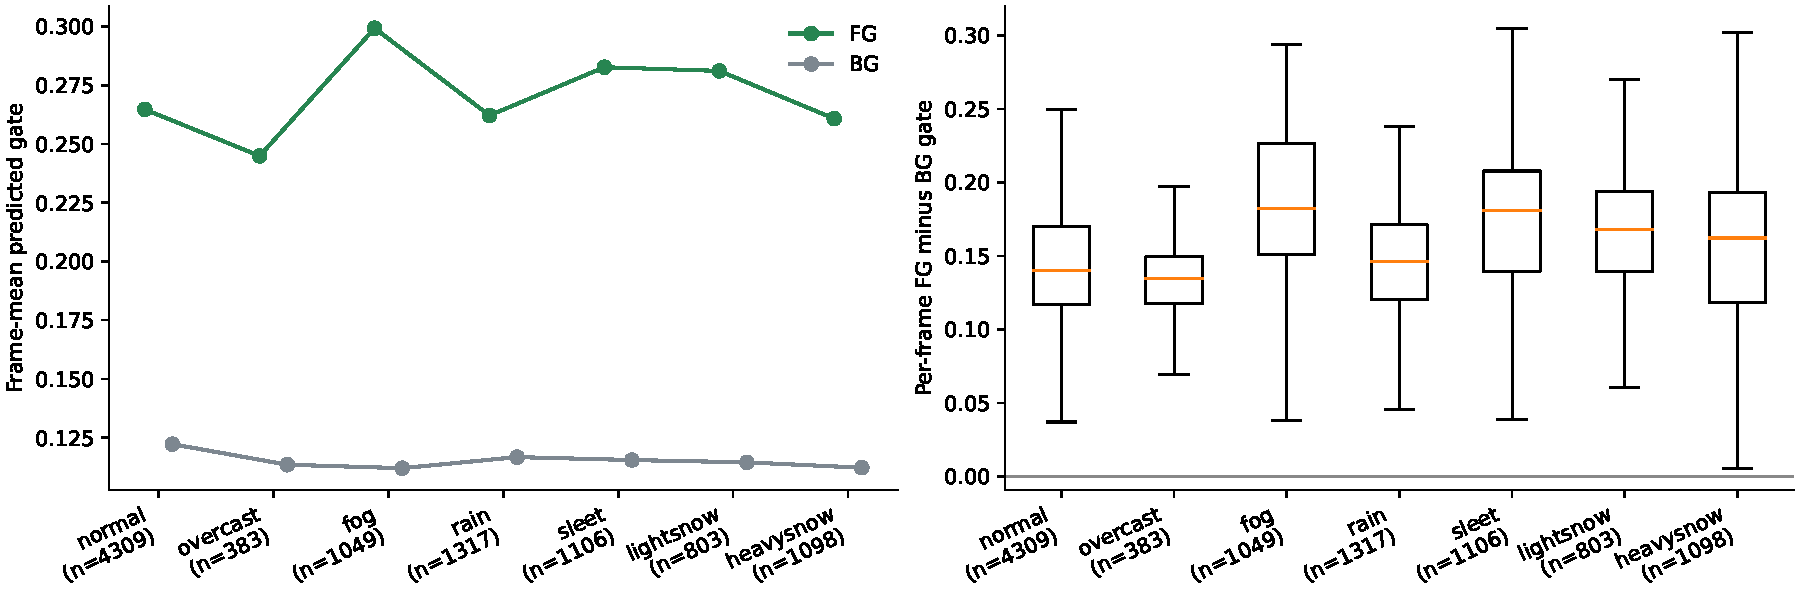
\includegraphics[width=\linewidth,height=.65\textheight,keepaspectratio]{assets/gate_all_weather_statistics.pdf}
\caption{Full-test foreground/background gate statistics over 10,065 frames. Left: weather-group means of per-frame foreground and background gate averages, with frames weighted equally. Right: distributions of each frame\textquotesingle s foreground-minus-background mean, with outliers hidden in the display. GT-defined regions are applied after feature-based gate prediction. Across all frames, foreground/background means are 0.2701/0.1176, and 99.06\% of frames have a larger foreground mean. These observational weather groups differ in sequences and scene composition and do not isolate a causal weather effect.}
\label{fig:e-gate-statistics}
\end{figure}

\begin{figure}[t]
    \centering
    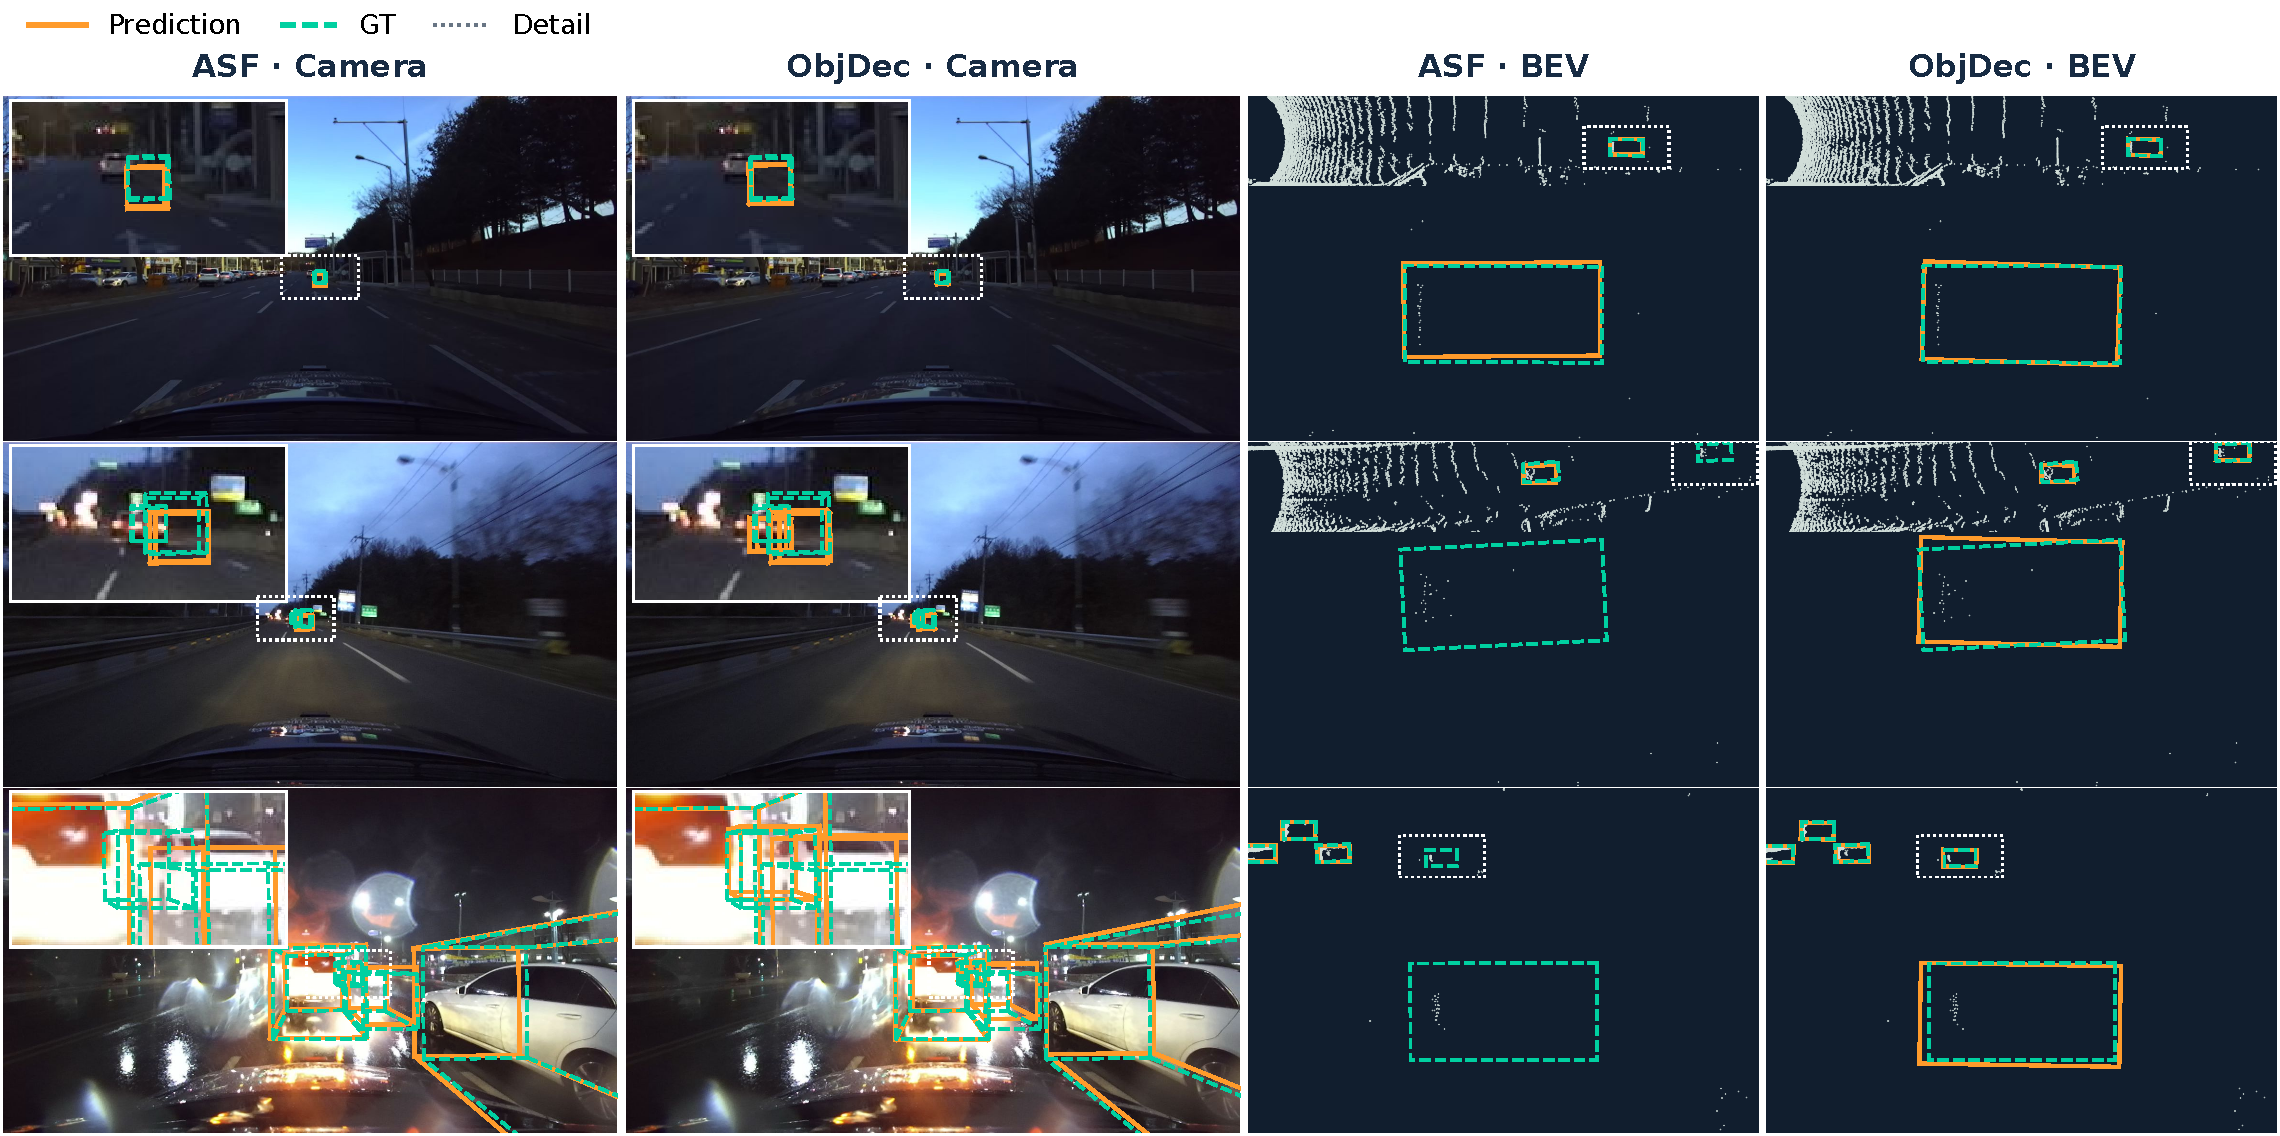
\includegraphics[width=\linewidth]{assets/figure5.pdf}
    \caption{Qualitative comparison of the released ASF checkpoint and ObjDec on identical K-Radar v1 test frames. The first two columns show calibrated camera projections with enlarged insets; the last two show full LiDAR BEV views above matched detail windows. Orange solid boxes denote Sedan predictions with scores above 0.3; green dashed boxes denote GT. Both methods use identical inputs, detection postprocessing, display thresholds, and camera/BEV crop windows. White dotted rectangles mark the enlarged regions. Full BEV views cover $x\in[0,72]$ m and $y\in[-6.4,6.4]$ m, while each detail window spans $12\times6$ m. For the highlighted GT, maximum 3D IoU among retained predictions changes from ASF to ObjDec as follows, from top to bottom: 0.572 to 0.719, 0.000 to 0.476, and 0.000 to 0.741. These values describe selected-object box overlap rather than AP; the middle example remains below IoU 0.5. Figure~\ref{fig:e3} includes an additional improvement and a localization counterexample.}
    \label{fig:e-comparison}
\end{figure}

\begin{figure}[p]
\centering
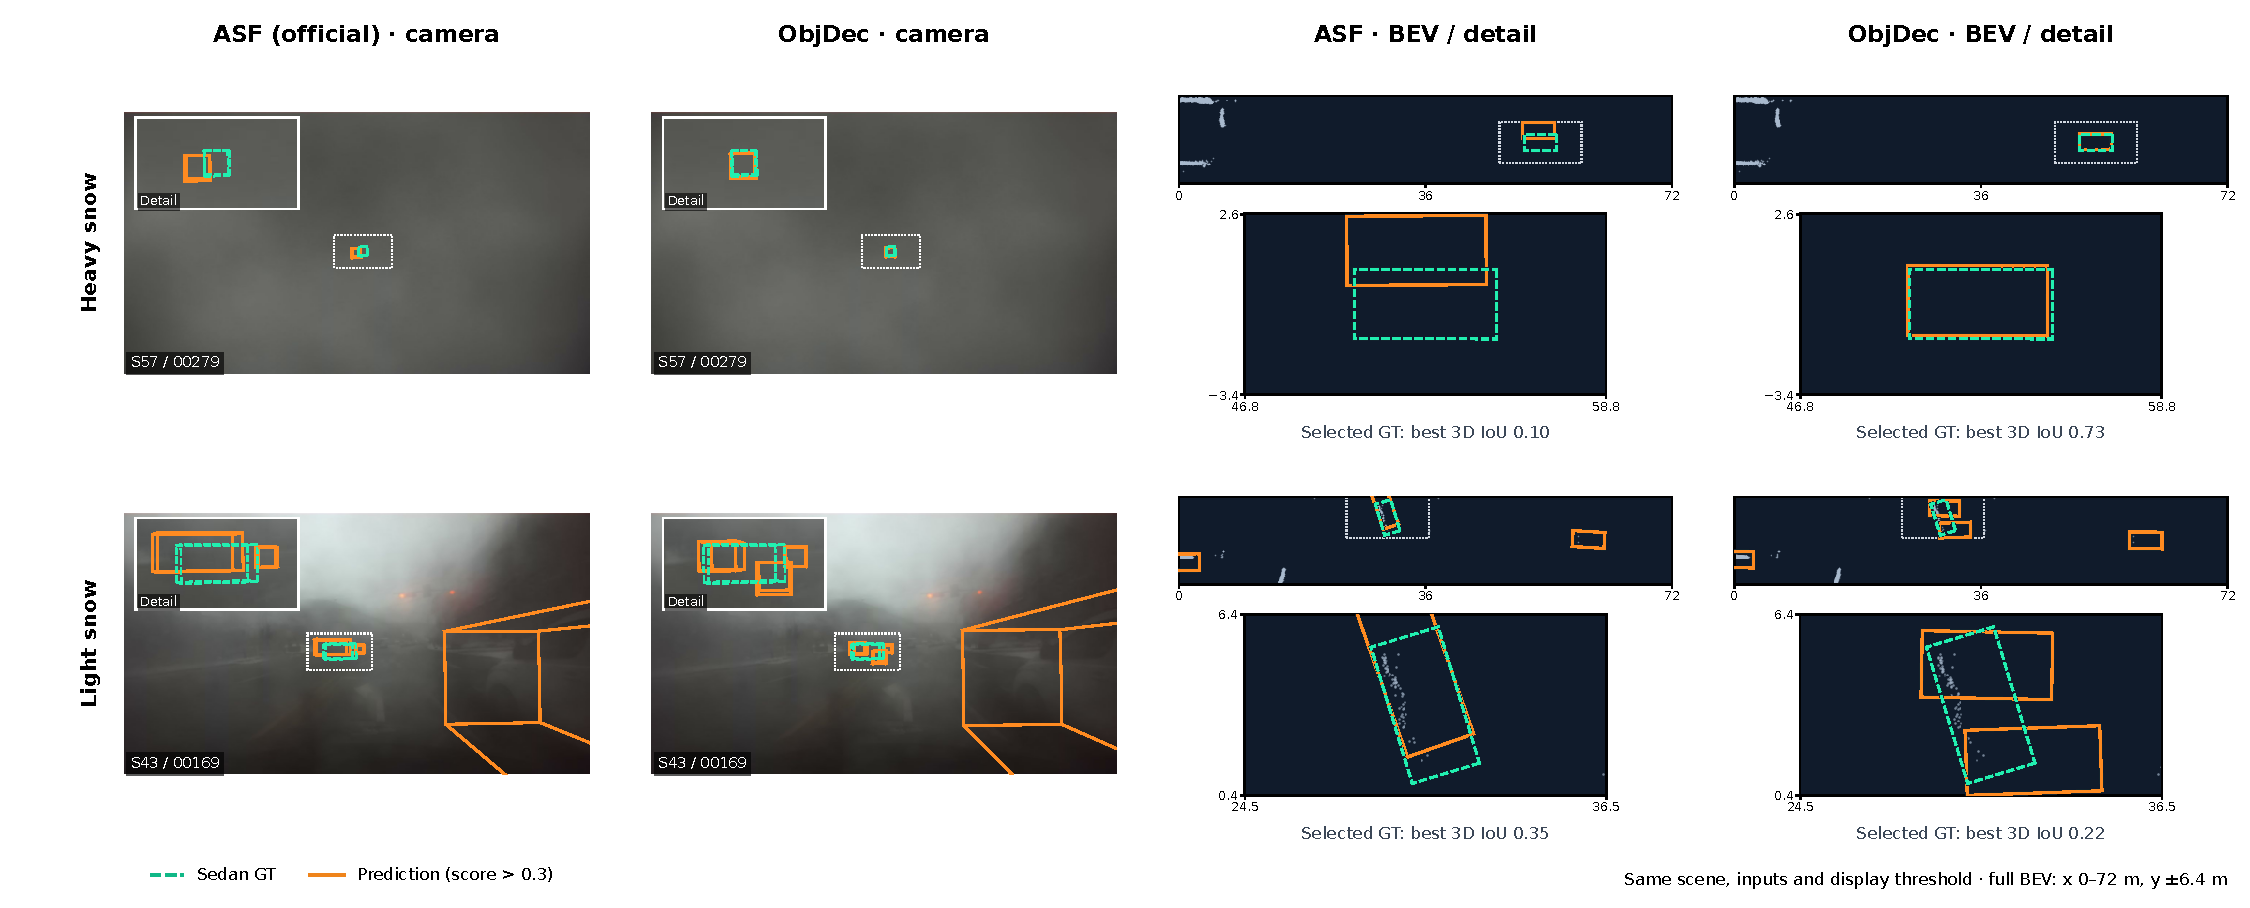
\includegraphics[width=\linewidth,height=.69\textheight,keepaspectratio]{assets/snow_counterexample.pdf}
\caption{Additional paired detections from the released ASF checkpoint and ObjDec. Green dashed boxes are GT and orange solid boxes are predictions with score>0.3; both methods use identical camera projections and detail windows. The selected heavy-snow object's maximum geometric 3D IoU increases from 0.095 to 0.728, whereas the light-snow object's decreases from 0.354 to 0.223. The latter also appears in the seven-weather appendix gate visualization, where locally high foreground response coexists with poorer localization. Foreground-related activation does not replace final box regression. Displayed IoUs describe selected-object overlap rather than AP.}
\label{fig:e3}
\end{figure}

